\documentclass{beamer}
\usepackage[utf8]{inputenc}
\usepackage{default}
% Texto Justificado
\usepackage{ragged2e}
\justifying
%  Tema Frankfurt
\usetheme{Frankfurt}

% Slides Negros (Pensar melhor nessa opção, pois pode dificultar a leitura)
%\usecolortheme{structure}

%%%%%%%%%%%%%%%%%%%%%%%%%%%%%%%%%%%%%%%%%%%%%%%%%%%%%%%%%%%%%%%%%%%%%%%%%%%%
% Informações gerais da apresentação
%%%%%%%%%%%%%%%%%%%%%%%%%%%%%%%%%%%%%%%%%%%%%%%%%%%%%%%%%%%%%%%%%%%%%%%%%%%%
\title[TCC]{Implantação e Análise de serviço Web Proxy Cache em Infraestruturas de Computação na Nuvem}
\author{Luís Eduardo Tenório Silva\\\textit{lets@cin.ufpe.br}\\Orientador: Almir Pereira Guimarães\\\textit{almirguimaraes@yahoo.com.br}}
\date[18/12/13]{18 de Dezembro de 2013}
\logo{
    
\includegraphics[height=1cm,keepaspectratio]{imagens/ufal.jpg}
    
\includegraphics[height=1cm,keepaspectratio]{imagens/comp.png}    
}

% Estruturação:
%    1- Definição de computação na nuvem
%    2- Motivação (Computação em nuvem): porque utilizar computação na nuvem.
%    3- Definição de proxy cache
%    4- Motivação (proxy cache): porque utilizar proxy cache.
%    5- Computação em nuvem + proxy cache (Trabalhos realizados) OBS: Pesquisar no IEEE para definir a data onde apareceu a junção dos conceitos.
%    6- Problemática:
%    Como realiar essa junção? Apresentar em números...OBS: Apresentar agora os problemas das diversas configurações
%    Como deve ser configurado para apresentar melhores resultados? DEPENDE DA MÉTRICA A SER OBSERVADA
%    7- Proxy cache:
%    - Tipos
%    - Arquiteturas
%    - Protocolos Inter cache
%    - Cache hit e cache miss
%    Cloud Computing:
%    - Características
%    - Categorias
%    - Virtualização
%    Arquiteturas OBS: Descrever cloud+proxy e começar a falar como será realizado a simulação do tráfego
%    Cenários
%    Resultados
%    Considerações finais
% 
\begin{document}
%   Título do trabalho
    \frame{\titlepage}

    \frame{\footnotesize{\tableofcontents}}
%   1- Definição de computação na nuvem
    \section{Computação na nuvem}
    \setbeamercovered{transparent}
    \begin{frame}
      \frametitle{Computação em nuvem}
     % \begin{block}{Definição abrangente}<1-| alert@1>
     % \textit{Hardwares de grande escala distribuídos geograficamente e infra-estrutura de software composto de recursos heterogêneos de rede compartilhado por várias organizações administrativas que são coordenados para fornecer transparência, confiabilidade, abrangência e suporte computacional persistente para uma grande variedade de aplicações.} (Miguel et
%al , 2004)
   % \end{block}    
    \begin{block}{Definição}<1- | alert@2>
      \textit{Forma de computação distribuída em que um "super computador virtual", composto de um conjunto de computadores de baixo
acoplamento interligados em rede, agindo em conjunto para realizar grandes tarefas.} (Buyya et al. 2009)
     \end{block}       
    \end{frame}
    \setbeamercovered{invisible}
%   2- Motivação (Computação em nuvem)
    \section{Motivação (Computação em nuvem)}
    \begin{frame}
      \frametitle{Motivação}
      Por que utilizar computação na nuvem?
      \begin{itemize}
       \item <2->Diversos serviços migrando para a internet e para a nuvem (Email, Editores de texto, Ambientes de desenvolvimento etc).
       \item <3->Economia de recursos
       \item <4->Controle maior do serviço (Elasticidade, pool de recursos...)
      \end{itemize}
    \end{frame}
%   3- Definição Proxy Cache
    \section{Web Proxy Cache}
    \begin{frame}
      \frametitle{Web Proxy Cache}
      \begin{block}{Definição}
	\textit{O cacheamento de páginas web e arquivos disponíveis em servidores web remotos, permitindo o acesso mais rápido e
confiável de clientes da rede local.} (Elvis Pontes 2010)
      \end{block}
    \end{frame}
%   4- Motivação (Proxy cache)
    \section{Motivação (Web Proxy Cache)}
    \begin{frame}
      \frametitle{Motivação}
      Por que utilizar Web Proxy Cache?
      \begin{itemize}
       \item <2-> Acesso rápido e seguro
       \item <3-> Controle de acesso a conteúdo
       \item <4-> Economia de recursos (Largura de banda, processamento de pacotes)
      \end{itemize}
    \end{frame}
%   5- Computação em nuvem + proxy cache (Trabalhos realizados)
    \section{Computação na nuvem + Web Proxy Cache}
    \begin{frame}
     \frametitle{Computação na nuvem + Web Proxy Cache}
     Primeiro trabalho no IEEE a relacionar Computação na Nuvem e Web Proxy Cache
     \begin{figure}
      \centering
      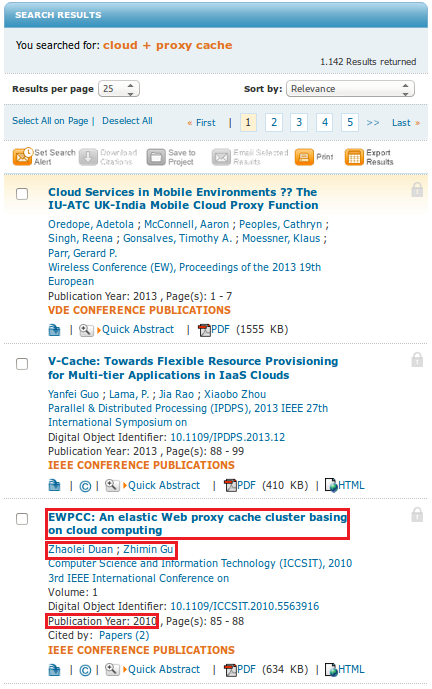
\includegraphics[scale=0.4]{imagens/pesquisa2.jpg}
      \caption{IEEE Explorer}
     \end{figure}

    \end{frame}
%   6- Problemática
%    Como realiar essa junção? Apresentar em números...OBS: Apresentar agora os problemas das diversas configurações
%    Como deve ser configurado para apresentar melhores resultados? DEPENDE DA MÉTRICA A SER OBSERVADA
    \section{Problemática}
    \begin{frame}
     \frametitle{Problemática}
     \begin{itemize}
       \item Como juntar os conceitos de computação na nuvem com web proxy cache?
       \item Qual deve ser a configuração do serviço para que apresente o melhor resultado possível?
      \end{itemize}
    \end{frame}
%    7- Proxy cache:
%    - Tipos
%    - Arquiteturas
%    - Protocolos Inter cache
%    - Cache hit e cache miss
    \section{Proxy Cache}
    \subsection{Cache hit e Cache miss}
    \begin{frame}
      \frametitle{Cache hit e Cache miss}
      Cache Hit: Quando o objeto solicitado for encontrado no cache.
      Cache Miss: Quando o objeto não é encontrado no cache.

      \begin{figure}
       \centering
       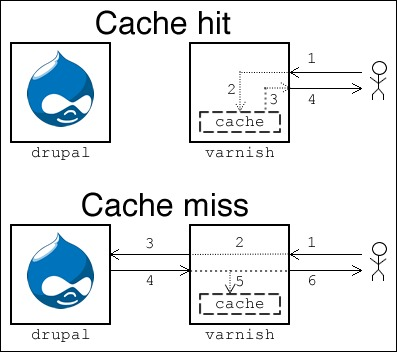
\includegraphics[scale=0.4]{imagens/cachehit.jpg}
       \caption{Cache hit e Cache miss}
      \end{figure}

    \end{frame}

   \subsection{Arquiteturas}
    \begin{frame}
      \frametitle{Arquiteturas}
      Árvore: Hierarquia Pai/Filho/Irmãos.\\
      \begin{figure}
       \centering
       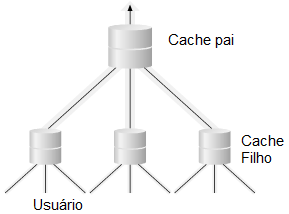
\includegraphics[scale=0.3]{imagens/hierarquia.png}
       \caption{Hierarquia}
      \end{figure}

      Malha: Abolição de hierarquias.

      \begin{figure}
       \centering
       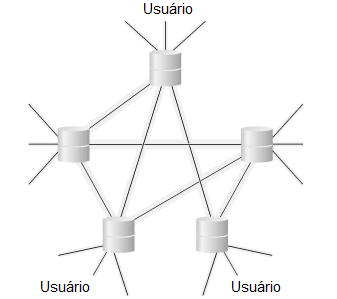
\includegraphics[scale=0.3]{imagens/mesh.png}
       \caption{Malha}
      \end{figure}
  
    \end{frame}

    \subsection{Protocolos Inter-cache}
    \begin{frame}
      \frametitle{Protocolos Inter-cache}
      Responsáveis pela comunicação entre diversos caches.
      \begin{itemize}
       \item ICP (Internet Cache Protocol): Leve
       \item CARP (Cache Array Routing Protocol): Balanceamento de carga       
       \item Digest: Resumo de cache
      \end{itemize} 
    \end{frame} 

%    Cloud Computing:
%    - Características
%    - Categorias
%    - Virtualização
    \section{Computação na nuvem}  
    \subsection{Categorias}    
    \begin{frame}
      \frametitle{Categorias (Computação na nuvem)}
      \begin{itemize}
       \item SaaS (Software como Serviço)
       \item PaaS (Plataforma como Serviço)
       \item \textbf{IaaS} (Infraestrutura como Serviço)
      \end{itemize}
    \end{frame}

    \subsection{Virtualização}
    \begin{frame}
     \frametitle{Virtualização}
     Virtualização consiste na emulação de ambientes completos (Singh 2004), podendo ser constituídos por sistema operacional, rede, software, armazenamento, entre outros.\\
     Ambientes emulados são também chamados de \textbf{máquinas virtuais}.
    \end{frame}

    \begin{frame}
     \frametitle{Tipos}
     \begin{itemize}
      \item Virtualização total: O hypervisor emula todo hardware que será utilizada pelas máquinas virtuais.
      \item Para-virtualização: O kernel do sistema operacional das máquinas virtuais é alterado.
      \item Virtualização a nível de sistema operacional: O kernel do sistema operacional da máquina virtual e física são alterados.
     \end{itemize}
    \end{frame}

%    Arquiteturas OBS: Descrever cloud+proxy e começar a falar como será realizado a simulação do tráfego
    \section{Arquitetura}
    \begin{frame}
     \frametitle{Arquitetura}
     \begin{figure}
      \centering
      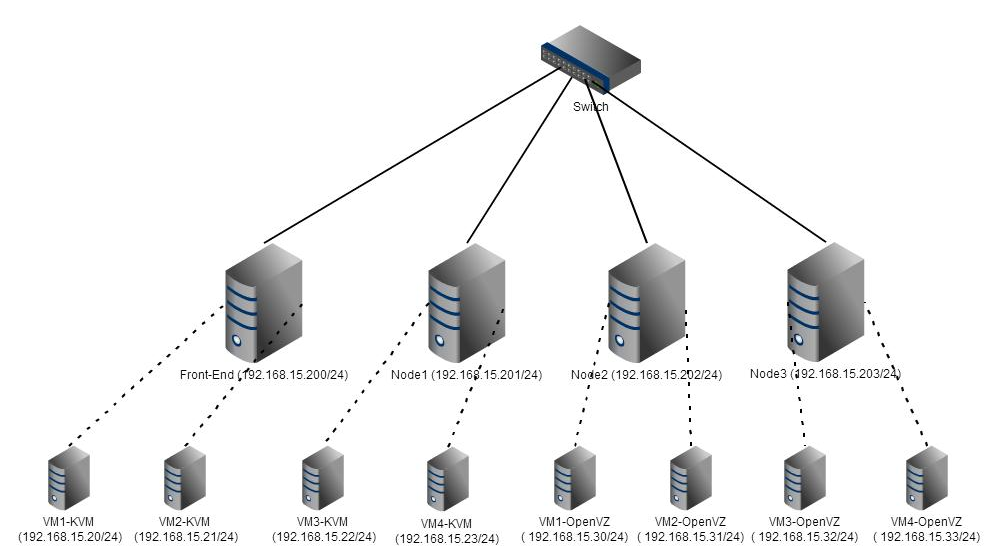
\includegraphics[scale=0.4]{imagens/arquiteturanuvem.png}
      \caption{Arquitetura da nuvem}
     \end{figure}
    \end{frame}

    \begin{frame}
     \frametitle{Problemática}     
     Qual deve ser a configuração do serviço para que apresente o melhor resultado possível?\\
     \textcolor{green}{Depende das métricas que estão sendo observadas}
    \begin{itemize}
     \item Proxy Cache\textbf{Taxa de acerto:} ${Cache Hit\over(Cache Hit + Cache Miss)}$
     \item Computação na nuvem: Disponibilidade do serviço
    \end{itemize}
    \end{frame}

    \begin{frame}
      \frametitle{Resposta}
      \huge{Uso de simulação de tráfego de alta recorrência.(Tráfego mais próximo de um ambiente real)}
    \end{frame}

    \section{Simulação}
    \begin{frame}
     \frametitle{Simulação}
      Uso do WebPolygraph para simulação de tráfego.
      \begin{itemize}
       \item Uso de 75\% de recorrência (Alta recorrência).
       \item Uso de distribuição de probabilidade para simulação do tráfego e tamanho dos objetos (Pareto e Zipf).       
      \end{itemize}

      \begin{figure}
       \centering
       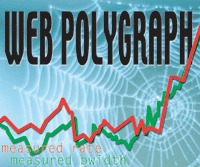
\includegraphics[scale=0.5]{imagens/webpolygraph.jpg}
       \caption{WebPolygraph}
      \end{figure}
    \end{frame}

    \begin{frame}
     \begin{figure}
      \centering
      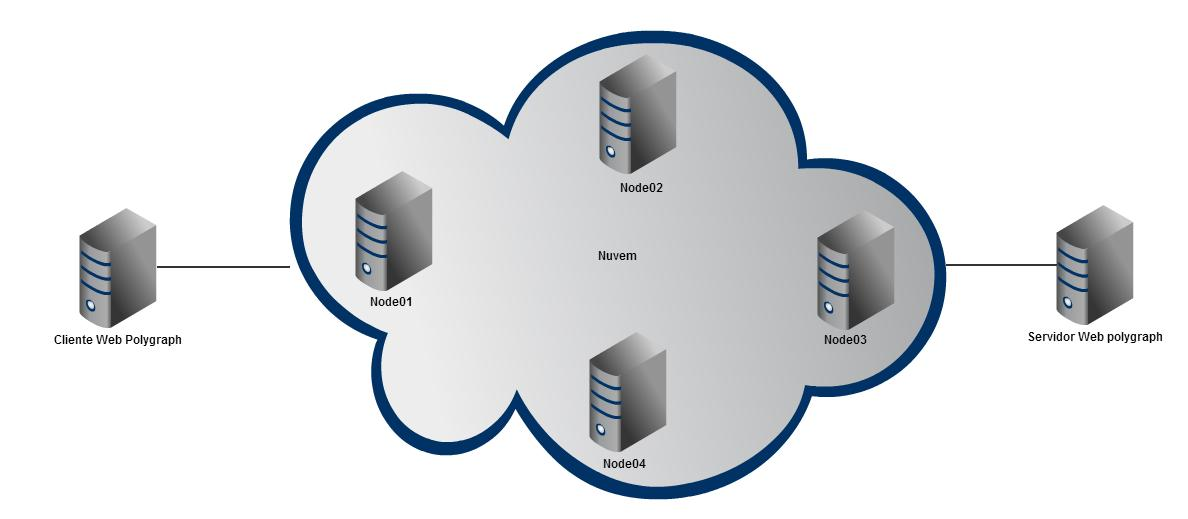
\includegraphics[scale=0.2]{imagens/simulador.jpg}
      \caption{Arquitetura na nuvem com simulador}
     \end{figure}
    \end{frame}

%    Resultados
    \section{Resultados}
    \begin{frame}
     \frametitle{Resultados}     
    \begin{figure}
      \centering
      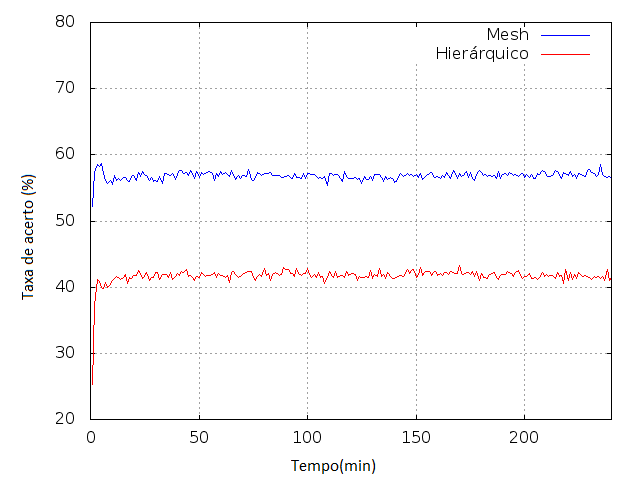
\includegraphics[scale=0.4]{imagens/meshhierarquico.png}
      \caption{Resultado Mesh(Malha) x Hierarquco}
    \end{figure}
    \end{frame}

    \begin{frame}
     \frametitle{Resultados}     
     \begin{figure}
      \centering
      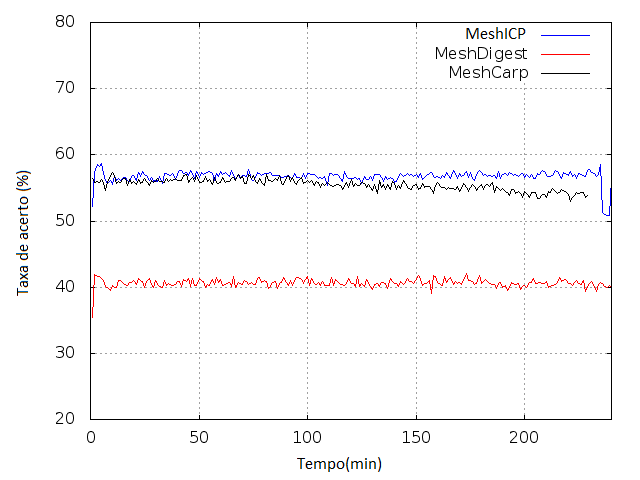
\includegraphics[scale=0.4]{imagens/protocolos.png}
      \caption{Resultado ICP x Digest x Carp}
      \end{figure}
    \end{frame}

    \begin{frame}
     \frametitle{Resultados}
      \begin{figure}
      \centering
      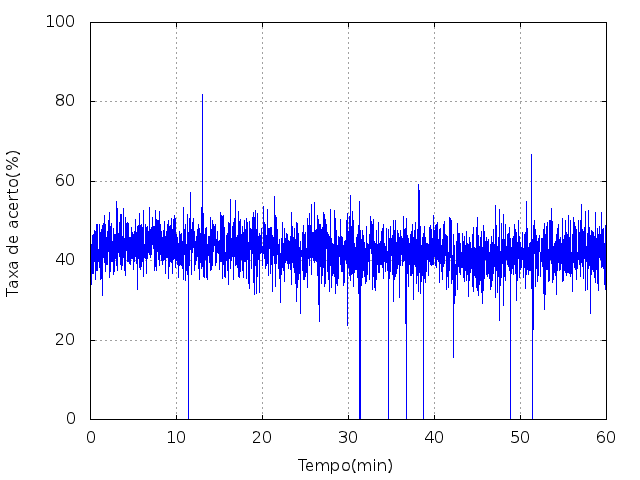
\includegraphics[scale=0.4]{imagens/grafico_openvz.png}
      \caption{Resultado OpenVZ}
      \end{figure}
    \end{frame}

    \begin{frame}
     \frametitle{Resultados}
      \begin{figure}
      \centering
      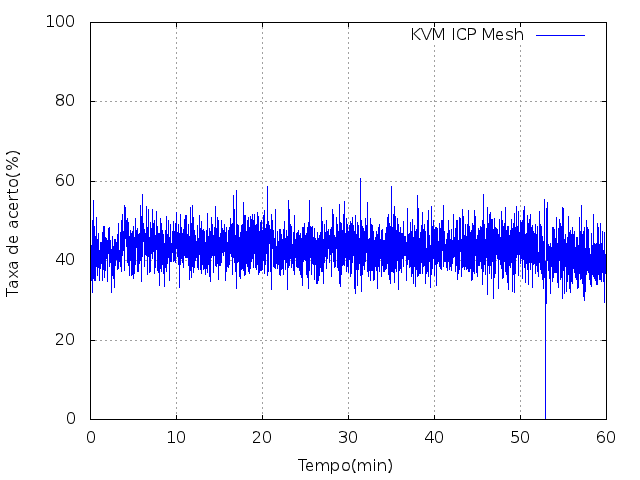
\includegraphics[scale=0.4]{imagens/kvm.png}
      \caption{Resultado KVM}
      \end{figure}
    \end{frame}

%    Considerações finais
    \section{Considerações Finais}
    \begin{frame}
     \frametitle{Considerações Finais}
    \end{frame}

\end{document}
